\subsubsubsubsection{Moving entity}
\begin{figure}[h]
\centering
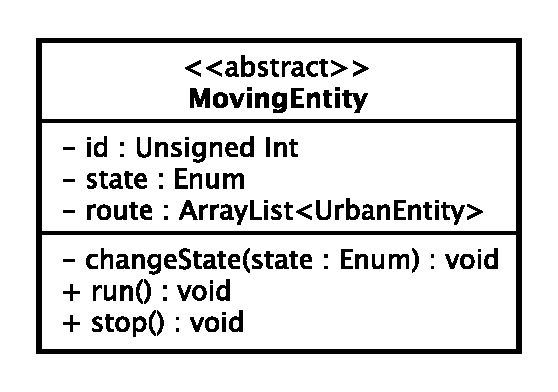
\includegraphics[scale=0.6,keepaspectratio]{sections/images/solution/moving_entity.eps}
\caption{App::Active::MovingEntity}
\label{fig:sd-app-movingentity}
\end{figure}
\begin{itemize}
  \item \textbf{Description} \\
    It represents an entity that moves through the city, consuming its 
route at each stretch treaded.
  \item \textbf{Attribute}
  \begin{itemize}
    \item \texttt{- id: Unsigned Int} \\
A unique identifier, useful to keep track of each entity.
    \item \texttt{- state: Enum} \\
The possible states of the entity \{ running, stopped \}.
    \item \texttt{- route: ArrayList<UrbanEntity>} \\
The route of urban entities that the entity has to tread.
  \end{itemize}
  \item \textbf{Operation}
  \begin{itemize}
    \item \texttt{- changeState(state: Enum)} \\
Change the entity state. This method is used internally by public methods to 
change the entity behaviour.
    \item  \texttt{+ run()} \\
Activates the entity which sets its state to \textit{running} and 
starts consuming its route.
    \item  \texttt{+ stop()} \\
Stops the entity which sets its state to \textit{stopped}.
  \end{itemize}
\end{itemize}
